\begin{figure}\label{fig:eval-success}
  \centering
    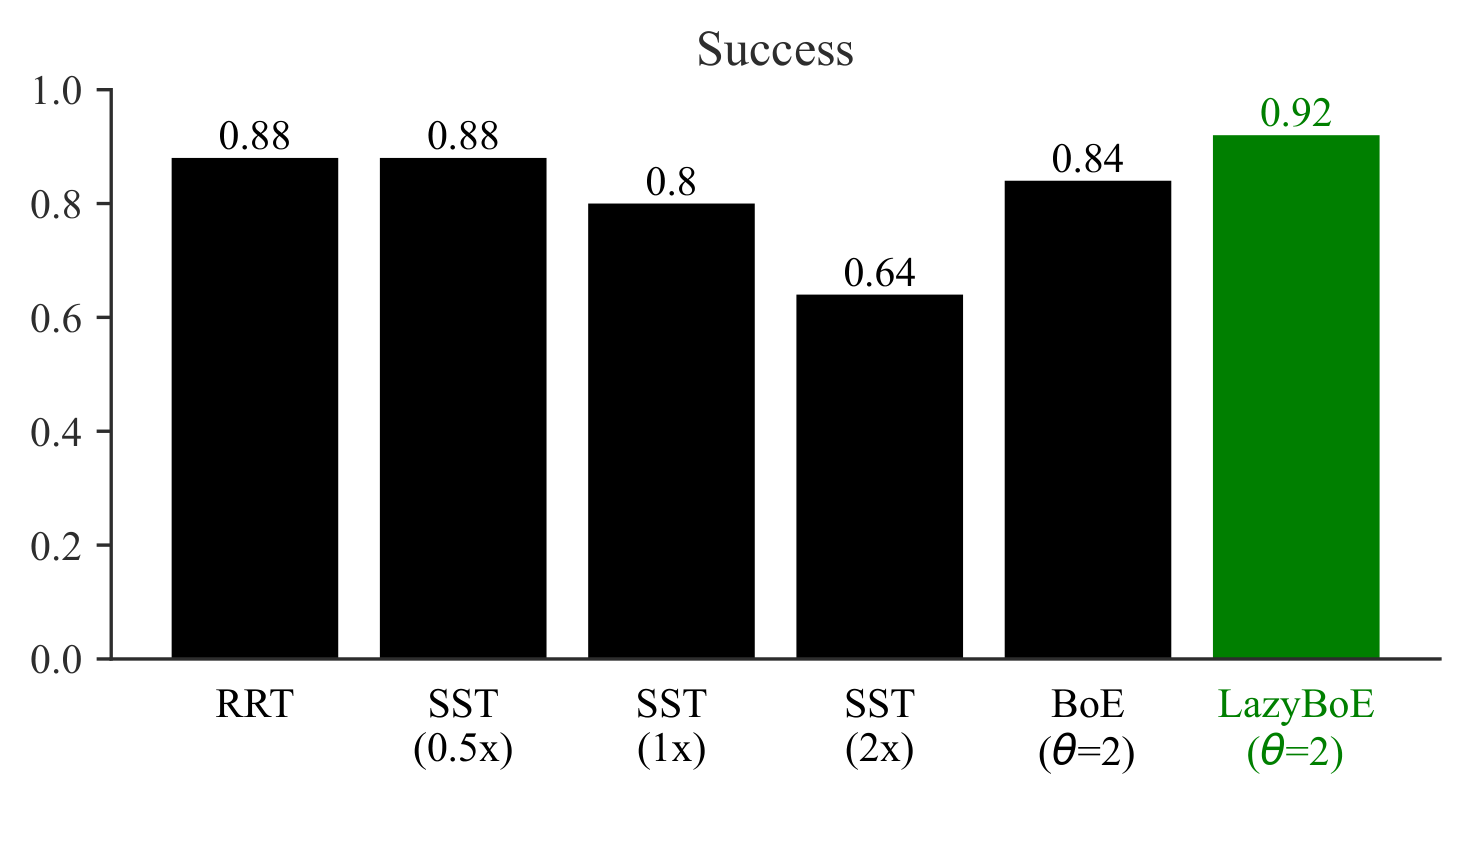
\includegraphics[width=\columnwidth]{assets/success_rate.png}
  \caption{Our algorithm has a higher success rate compared to the baselines owing to the exploration of a greater number of potential solutions (\cref{fig:eval-num_solutions}).}\label{fig:eval-success}
\end{figure}

\section{Conclusion and Discussion}\label{sec:discussion}

In this work, we presented \textsl{LazyBoE}, a multi-query approach to kinodynamic motion planning that takes advantage of lazy propagation and collision checking to outperform existing baselines in a number of key metrics. Specifically, our method reduces planning time and demonstrates a high success rate, given its ability to explore a wider range of solutions.
However, our method faces certain limitations. The varying control sampling for a given Monte Carlo propagation introduces jitter into the trajectory which has to be smoothed with a low-pass filter before real-world execution. Future work can explore biased sampling techniques that consider the history of control states.
Due to memory limitations, \textsl{LazyBoE} is confined to a limited subset of the robot's state and control spaces.
Scaling the approach to cover the entire robot workspace is a pressing challenge, stemming from memory constraints, especially when planning dynamically-feasible trajectories that may involve higher-order derivatives of the state space variables. While strategies such as selective loading or using a database could alleviate this, they require significant engineering optimizations.

Beyond the engineering required to scale this method, we also intend to explore
application-centric extensions, such as planning for heavy payloads, liquid transport, and nonprehensile manipulation,
which can benefit from assigning task-specific weights to edges for more biased, multi-query exploration.
While our implementation focuses on kinodynamic planning for robotic manipulation, the foundational principles of our planner are designed with broader applicability in mind. Generalizing the planner to accommodate a wider array of kinodynamic planning problems, beyond the realm of robotic manipulation, represents a promising direction for future work.
